\documentclass[final,5p,times,twocolumn]{elsarticle}
\usepackage[T1]{fontenc}
\renewcommand{\ttdefault}{lmtt}
\usepackage{microtype,graphicx,booktabs,amsmath,amssymb,amsthm,array,tabularx,longtable,multirow}
\usepackage{xcolor,tikz,pgfplots,enumitem,placeins,xurl}
\usetikzlibrary{arrows.meta,positioning,calc,fit,matrix,backgrounds}
\pgfplotsset{compat=1.18}
\usepackage[hypertexnames=false]{hyperref}
\hypersetup{hidelinks,pdfauthor={Chengzhan Li},pdftitle={Phase-Scoped Query Layouts for Reference-Preserving Speculative Decoding},pdfsubject={Reconstructed author-review manuscript v0.15.0; not submitted}}
\definecolor{target}{HTML}{426B8B}
\definecolor{draft}{HTML}{B07B43}
\definecolor{qualified}{HTML}{3E725E}
\definecolor{aux}{HTML}{6B7075}
\definecolor{light}{HTML}{EDF1F3}
\newcommand{\QB}{\mathrm{QB}}
\newcommand{\PQ}{\mathrm{PQ}}
\newcommand{\GS}{\mathrm{GS}}
\newcommand{\MQ}{\mathrm{MQ}}
\newcommand{\kw}[1]{\texttt{#1}}
\newcommand{\same}{\textcolor{qualified}{\ensuremath{=}}}
\newcommand{\diff}{\textcolor{draft}{\ensuremath{\ne}}}
\newtheorem{proposition}{Proposition}
\setlength{\emergencystretch}{2em}
\setlength{\tabcolsep}{4pt}
\renewcommand{\arraystretch}{1.14}
\setlist{nosep,leftmargin=*}
\makeatletter
\def\ps@pprintTitle{\let\@oddhead\@empty\let\@evenhead\@empty\def\@oddfoot{\hfil\thepage\hfil}\let\@evenfoot\@oddfoot}
\makeatother
\tikzset{box/.style={draw=aux,rounded corners=1pt,align=center,inner sep=5pt,font=\small},flow/.style={-{Latex[length=2mm]},line width=.55pt,draw=aux}}

\usepackage{flushend}
\begin{document}
\begin{frontmatter}
\title{Phase-Scoped Query Layouts for Reference-Preserving Speculative Decoding}
\author{Chengzhan Li\corref{cor1}}
\ead{chengzhan.li@std.uestc.edu.cn}
\cortext[cor1]{Corresponding author.}
\address{University of Electronic Science and Technology of China, Qingshuihe Campus,\\
No. 2006 Xiyuan Avenue, West Hi-Tech Zone, Chengdu, Sichuan 611731, China}
\begin{abstract}Speculative decoding changes the target's execution geometry, which can alter a quantized runtime's greedy output even when the acceptance protocol is correct. We introduce phase-scoped query-batch attention (QB), a graph transformation that places query columns on a batch axis while retaining batched projections and feed-forward computation. Query and mask views preserve native indexing semantics; role/phase guards and a layout-sensitive graph cache apply the transformation during target prefill and continuation. On 24 captured CUDA attention contexts, QB matches explicit per-query attention (PQ) bitwise at QK, softmax and AV. A separate three-family CUDA confirmation preserves complete registered outputs, and all seven arms qualify in a 2,016-request implementation study with an EOG-or-128-token endpoint. Speculative request-time ratios are 1.022--1.068 for PQ/QB and 1.463--2.176 for global serialization/QB; ratios above one favor QB. Adding a draft to the repaired path benefits Qwen3 and Llama but slows SmolLM2. Complementary Vulkan interventions show that prefill partitioning can change projection outputs and that retained KV differences can select later trajectories under a validated common receiver. These results identify a design choice for the evaluated quantized stack: constrain attention geometry while retaining other batching, and assess repair cost separately from draft benefit.
\end{abstract}
\begin{keyword}
speculative decoding \sep execution geometry \sep numerical consistency \sep runtime graph transformation \sep quantized inference
\end{keyword}
\end{frontmatter}
\section{Introduction}
\label{sec:intro}
Speculative decoding proposes several tokens with a draft model and verifies them with a target, reducing the number of sequential target invocations when proposals are accepted~\cite{leviathan2023}. The execution change is not merely a reduction in calls. Verification processes several query positions together, while ordinary greedy decoding processes one continuation position at a time. In a finite-precision implementation, two mathematically equivalent organizations of that work can produce different scores and, at a close decision boundary, different tokens. A correct acceptance protocol therefore does not by itself establish reproduction of a particular deployed greedy reference.

This distinction matters when a runtime optimization must preserve an existing regression baseline. We study that explicit requirement: the target weights, input formatting, sampler, stopping rule and ordinary execution recipe define a registered reference. A candidate is eligible for a reference-preserving latency comparison only when its complete native output satisfies the same requirement. We do not equate reference preservation with answer correctness, statistical sampling equivalence, or equality of every internal floating-point value. An implementation can be repeatable yet consistently disagree with this reference.

A direct response is to serialize the target computation. That removes opportunities for batching well beyond the operations that need numerical control. Our central observation is that \emph{the organization of attention queries can be separated from the batching of the surrounding target network}. Attention can retain one query column per batch instance while projection, output projection and feed-forward operators continue to process several tokens together. This is a concrete graph-design choice: it changes the attention representation without introducing a new draft algorithm or a new arithmetic kernel.

We implement this choice as a \emph{phase-scoped query layout}. After the runtime's existing permutations, the query view changes from $(d,q,h, 1)$ to $(d, 1,h,q)$. A corresponding mask view preserves each query's admissible keys, and shared K/V remain associated with the same logical stream. The method also includes two runtime obligations. A role/phase guard activates the layout in the intended target phases even when observation is disabled; a graph-reuse key prevents a cached unconstrained topology from bypassing that guard. These obligations are part of the method, not incidental instrumentation.

The empirical argument separates three questions. First, does the transformation have the intended numerical behavior on identical attention inputs? Second, does the complete decoder preserve its registered output? Third, is this implementation cheaper than another implementation that passes the same output test? The first two cannot substitute for each other: identical sampled operators do not establish a whole-model theorem, and matching tokens can conceal numerical differences. The third requires more than comparing a candidate with an unoptimized ordinary decoder. We compare query-batch attention with explicit per-query attention and target-global serialization, then separately measure whether adding a draft is worthwhile on the repaired path.

The CUDA results support all three questions within the tested scope. In 24 captured contexts, query-batch and per-query attention agree bitwise at QK, softmax and AV, whereas ordinary multi-query execution differs. A larger confirmation campaign checks Qwen3, SmolLM2 and Llama under a frozen target-phase configuration. A subsequent implementation campaign executes 2,016 complete requests across seven arms, with all arms meeting the common output requirement. Query-batch is cheaper in aggregate than per-query attention and global serialization in each family, although some per-task comparisons regress and the per-query advantage is small. Drafting remains unprofitable for SmolLM2. These are distinct findings: a less expensive repair need not make speculation profitable.

A separate Vulkan investigation tests the limit of an attention-centered explanation. Changing prefill partitioning at fixed context settings reproduces two historical output divergences. First-layer projection differences appear before later attention, and a validated boundary-state reconstruction shows that the affected suffix follows the retained KV source. This experiment is not a transfer of the CUDA query-batch patch. Instead, it explains why a layout method must state its admitted runtime conditions and validate state formation, rather than assume that attention is the only numerically sensitive operation on every backend.

The paper makes three contributions. \textbf{(1) A specified runtime transformation:} query and mask address mappings, K/V and grouped-query semantics, output ordering, phase activation and cache-reuse conditions define an implementable attention layout. \textbf{(2) Layered numerical and output evidence:} fixed-input operator replay and three-family complete-output qualification establish different, explicitly bounded properties. \textbf{(3) Same-reference implementation and state-boundary evaluation:} fair per-query/query-batch/serialized comparisons establish repair cost separately from draft value, while Vulkan partition and KV interventions delimit portability. We make no claim of a new sampling rule, a universal minimal constraint, or superiority to an external determinism system under a common workload.

\section{Reference Contract and Execution Model}
\label{sec:problem}
\subsection{What is held fixed}
Let $\rho$ identify a reference configuration: model and tokenizer bytes, prompt construction, numerical runtime and backend, sampler, context settings, stopping convention and ordinary execution recipe. For input $x$, define the observable endpoint
\begin{equation}
\mathcal O_\rho(x)=(\boldsymbol y,\boldsymbol e,n,y_{\rm last},s),
\label{eq:contract}
\end{equation}
where $\boldsymbol y$ is the full generated native token-ID array, $\boldsymbol e$ its EOG flags, $n$ its length, and $s$ the stop reason. For the principal new campaigns, generation ends at native EOG or cap128. Complete output here means complete under that registered window, not an arbitrarily long answer. Earlier campaigns with first-EOG endpoints and additional raw suffixes retain their original, weaker comparison scope in Supplement~S 7.

For an evaluation set $\mathcal X$ and its registered repetitions, empirical qualification requires $\mathcal O_c(x)=\mathcal O_\rho(x)$ for every required candidate/reference pair, as well as reference stability and complete records. Qualification is indexed by $\rho$ and $\mathcal X$: it is not a statement about all future inputs. A missing endpoint is not imputed; a divergent shorter response cannot qualify a latency ratio. Repeated measurements are not additional independent tasks.

Three levels of equality must remain separate. A tensor view may preserve mathematical values and indices while changing finite-precision evaluation. Selected operators may agree bitwise without proving agreement elsewhere in the network. Finally, identical output IDs may coexist with different logits and KV values. The method supplies a mathematical indexing argument and empirical numerical and endpoint tests, not a deduction that the first level guarantees the other two.

\subsection{A stateful speculative transaction}
A target context owns its KV state, sequence positions, pending sampled token or logits, and relevant sampler/loop state. A draft context owns separate state. In each speculative cycle, the draft proposes up to $k$ tokens; the target evaluates the pending token and proposal positions; acceptance, correction and any bonus determine the committed prefix. Rejected positions are reconciled before continuing. A sampled token may already be committed to the visible output but still be pending evaluation into KV. Resampling it or consuming it twice changes the transaction.

Our transformation does not change this protocol. It changes how admitted target attention work is represented. In particular, the measured CUDA candidate introduces no additional replay whose purpose is to repair numerical consistency; normal speculative verification and reconciliation still execute and are charged. This distinction prevents the phrase ``no replay'' from being mistaken for removal of target verification.

Microbatch capacity $U$, occupied query count $q$, caller width and output reservation are distinct. We use UB$n$ as shorthand for a configured microbatch capacity of $n$ tokens. A target-only continuation may occupy one query under either $U=1$ or $U=512$. A speculative caller can contain $k+1$ logical rows yet execute several physical micrographs. Output reservation affects the available result interface, not simply the number of active queries. The experimental arms record all four notions rather than treating a configured capacity as actual GPU work.

\subsection{The design problem}
For fixed $\rho$, our engineering goal is to reduce measured request time subject to qualification:
\begin{equation}
\min_{c\in\mathcal C_{\rm tested}} T_c
\quad\text{subject to}\quad
\mathcal O_c(x)=\mathcal O_\rho(x)\;(x\in\mathcal X).
\label{eq:designproblem}
\end{equation}
Equation~\eqref{eq:designproblem} defines a finite design comparison, not an optimizer or global optimum claim. The tested candidate set contains ordinary execution and three repair organizations: per-query attention (PQ), query-batch attention (QB), and global target serialization (GS). Each organization is assessed with and without a draft. The contribution is the specified QB implementation and its measured trade-off against these alternatives.

\section{Phase-Scoped Query-Layout Design}
\label{sec:method}
\subsection{Separating attention from target-wide batching}
Figure~\ref{fig:design} contrasts the three repair organizations. GS processes target rows one at a time throughout projection, attention and the feed-forward network. PQ retains batched surrounding work but explicitly constructs an attention subgraph for each query and concatenates the results. QB retains that local one-column organization through a view: queries become separate batch instances of the existing attention operators. It does not serialize the surrounding layers or construct a distinct attention subgraph per query.

\begin{figure*}[t]
\centering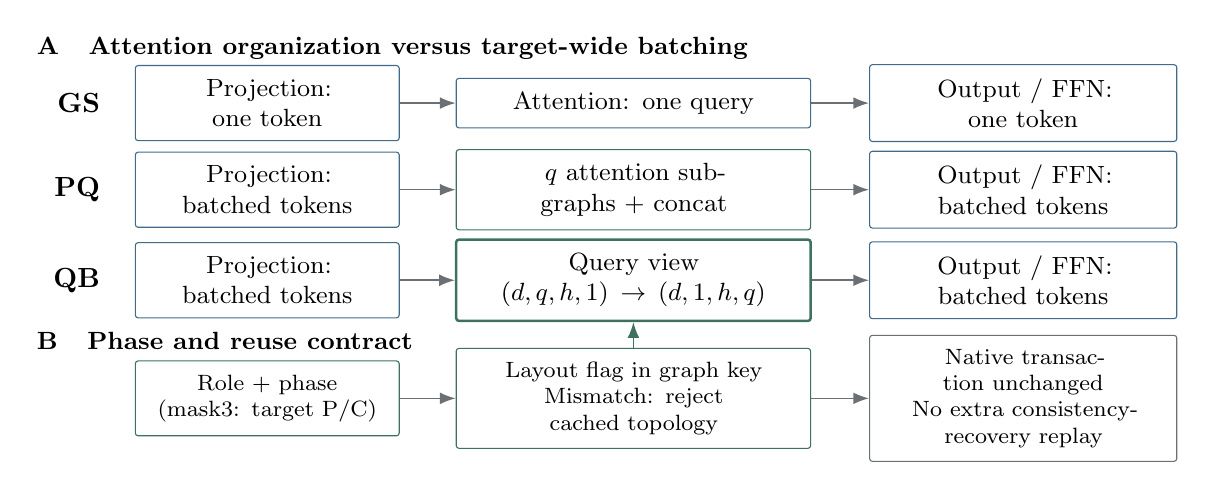
\begin{tikzpicture}[x=1cm,y=1cm,font=\small]
\node[anchor=west,font=\bfseries\small] at (0,4.05) {A\quad Attention organization versus target-wide batching};
\foreach \y/\lab in {3.35/GS,2.25/PQ,1.10/QB} {
 \node[anchor=east,font=\bfseries] at (1.05,\y) {\lab};
}
\node[box,draw=target,text width=3.0cm] (g1) at (3.05,3.35) {Projection: one token};
\node[box,draw=target,text width=4.15cm] (g2) at (7.70,3.35) {Attention: one query};
\node[box,draw=target,text width=3.55cm] (g3) at (12.65,3.35) {Output / FFN: one token};
\node[box,draw=target,text width=3.0cm] (p1) at (3.05,2.25) {Projection:\\batched tokens};
\node[box,draw=qualified,text width=4.15cm] (p2) at (7.70,2.25) {$q$ attention subgraphs + concat};
\node[box,draw=target,text width=3.55cm] (p3) at (12.65,2.25) {Output / FFN:\\batched tokens};
\node[box,draw=target,text width=3.0cm] (b1) at (3.05,1.10) {Projection:\\batched tokens};
\node[box,draw=qualified,line width=.9pt,text width=4.15cm] (b2) at (7.70,1.10) {Query view $(d,q,h,1)\to(d,1,h,q)$};
\node[box,draw=target,text width=3.55cm] (b3) at (12.65,1.10) {Output / FFN:\\batched tokens};
\foreach \a/\b in {g1/g2,g2/g3,p1/p2,p2/p3,b1/b2,b2/b3}\draw[flow] (\a)--(\b);
\node[anchor=west,font=\bfseries\small] at (0,.33) {B\quad Phase and reuse contract};
\node[box,draw=qualified,text width=3.0cm,font=\footnotesize] (phase) at (3.05,-.40) {Role + phase\quad(mask3: target P/C)};
\node[box,draw=qualified,text width=4.15cm,font=\footnotesize] (cache) at (7.70,-.40) {Layout flag in graph key\\Mismatch: reject cached topology};
\node[box,draw=aux,text width=3.55cm,font=\footnotesize] (native) at (12.65,-.40) {Native transaction unchanged\\No extra consistency-recovery replay};
\draw[flow] (phase)--(cache);\draw[flow] (cache)--(native);
\draw[flow,qualified] (cache.north)--(b2.south);
\end{tikzpicture}

\caption{Three same-reference implementation alternatives. Boxes indicate logical graph organization, not measured kernel occupancy. QB changes the attention representation while keeping surrounding target computation batched. The lower control path makes the phase decision part of graph construction and reuse. Draft proposal and target reconciliation are unchanged across speculative arms.}
\label{fig:design}
\end{figure*}

The intervention point follows the native Q/K/V permutations in the non-flash attention builder. Let $d$ be the query/key channel dimension, $q$ the number of occupied queries, $h_Q$ the query-head count, and $n$ the key extent. Using the runtime's axis order, the input query has shape $(d,q,h_Q, 1)$. QB creates a four-dimensional view with shape $(d, 1,h_Q,q)$ and preserves the original query-column stride as the new fourth-axis stride. This is a view of the same input values, not a different projection or a re-encoding of the tokens.

\subsection{Address, mask and head semantics}
Write the original byte strides as $s_0,s_1,s_2,s_3$ and the base pointer as $b_Q$. For channel $i$, head $a$ and logical query $j$, the original address is
\begin{equation}
\operatorname{addr}_{\MQ}(i,j,a, 0)=b_Q+i s_0+j s_1+a s_2.
\end{equation}
The transformed view satisfies
\begin{equation}
\operatorname{addr}_{\QB}(i, 0,a,j)=b_Q+i s_0+a s_2+j s_1,
\label{eq:address}
\end{equation}
so it selects the same scalar. The singleton query-column stride is immaterial for access, but the implementation still supplies a valid native view descriptor. It must not invent a contiguous layout when the source is strided.

The mask is transformed in parallel from $(n,q, 1,1)$ to $(n, 1,1,q)$. For original mask strides $m_0,m_1$, query $j$ still reads $b_M+t m_0+j m_1$ for key index $t$. The original mask values, including padded or disallowed positions, are retained. Changing the view must not replace a query-dependent causal mask by a single shared column. Logical token positions are unchanged: the new batch coordinate labels queries in one sequence, not independently positioned sequences.

Let $\kappa(a)$ denote the native grouped-query head mapping from query head $a$ to a K/V head. Under an integral grouped-query ratio, the same mapping is used by all three organizations. K and V retain their native values, strides and single-stream ownership and broadcast over the new query-batch coordinate. In mathematical notation, for the already implemented scaling $\alpha$ and admissible mask $m$,
\begin{align}
 z_{tja}&=\alpha\sum_i K_{it\kappa(a)}Q_{ija}+m_{tj},\\
 p_{tja}&=\frac{\exp(z_{tja})}{\sum_u\exp(z_{uja})},\\
 O_{vja}&=\sum_t V_{vt\kappa(a)}p_{tja}.
\label{eq:attn}
\end{align}
These equations describe logical indices; the actual runtime may store or permute V differently. QB must retain that implementation's mapping rather than reinterpret V by this notation alone.

\begin{proposition}[Mathematical view equivalence]
For a supported single-stream attention graph, suppose Equation~\eqref{eq:address} and the corresponding mask mapping hold, K/V broadcasting preserves $\kappa$, operator parameters are unchanged, and output recombination restores query order. In exact arithmetic, QB and the original attention graph compute the same logical $O$ in Equation~\eqref{eq:attn}.
\end{proposition}
\begin{proof}
For each fixed $(j,a)$, both representations select identical Q, K, V and mask values. The sums range over the same channel and key indices, and softmax is normalized over the same keys. The batch label in QB separates query instances but changes neither their operands nor their logical dependence. Recombination restores $(v,j,a)$ order. Thus every logical output value agrees in exact arithmetic. This argument makes no assertion about floating-point association, selected device algorithms or numerical equality of other target operators.
\end{proof}

After QK, softmax and AV, the native contiguous recombination restores the target's expected query/head order before its batched output projection. PQ realizes the same mathematical separation by slicing one query and its mask column per subgraph. The question tested later is whether QB matches PQ's \emph{observed numerical execution} without paying for the same subgraph structure.

\subsection{Admission conditions are part of the method}
The evaluated build admits one sequence/KV stream, non-flash attention, supported Qwen3 or dense Llama-family graph paths, compatible head dimensions, an integral GQA ratio, F32 query/mask values and F16 K/V. At most four queries are occupied in the current QB study. Attention bias, sinks and MLA value projections are excluded by the relevant source guards; other positional-bias schemes or unsupported strides require separate handling and validation. The mask may contain padded columns, but its first $q$ logical query columns and original key extent must be represented correctly.

These are not cosmetic restrictions. Additional streams require distinguishing a true sequence-batch dimension from the new query dimension. Biases or sinks must preserve their own broadcasting semantics. A fused attention kernel may choose a different numerical and memory schedule, and cannot inherit this non-flash result. A wider view can be mathematically legal yet numerically fail the registered reference. The implementation therefore rejects unsupported cases rather than advertising unconditional preservation. A separate historical wider-geometry build is evidence of a boundary, not an extension of the current four-query certificate.

\subsection{Phase binding and graph-cache consistency}
The transformation is selected by a process-fixed four-bit mask: target prefill, target continuation, draft prefill and draft continuation have bits 1, 2, 4 and 8. Mask 3 enables the two target phases. A scoped guard derives the active flag from the current role and phase, places that flag in graph parameters, and restores its prior value on exit. New requests reset the phase to prefill. Crucially, this guard executes before the observation-disabled fast path returns to native decoding; turning off a diagnostic callback must not disable the repair.

Graph caching creates a second obligation. Two calls can share nominal capacity and tensor extents yet require different attention layouts. The active-layout flag therefore participates in the reuse check. A mismatch rejects reuse and requires an appropriate graph. The implementation choice (QB, PQ or GS) is fixed within each process, so it cannot silently change under an already cached graph. The relevant design pattern is summarized in Table~\ref{alg:scope}; it is a description of deterministic dispatch, not automatic constraint search.

\begin{table}[t]
\caption{Phase-scoped dispatch and reuse obligations.}
\label{alg:scope}
\begin{tabularx}{\columnwidth}{@{}rX@{}}\toprule
1 & On request reset, establish target/draft ownership and set phase to prefill.\\
2 & Compute the role/phase bit and save the previous scope flag.\\
3 & Set the active flag before both observed and unobserved decode paths.\\
4 & If cached topology's layout flag differs, reject reuse.\\
5 & For an active supported attention graph, apply Q/mask views, native QK--softmax--AV and ordered recombination.\\
6 & Otherwise retain the declared untransformed graph or reject an unsupported active case.\\
7 & Complete native acceptance/state updates and restore the prior scope flag.\\\bottomrule
\end{tabularx}
\end{table}

The guards do not assert that every non-attention operation is batch-invariant. They preserve its batching and rely on complete output qualification under the tested numerical stack. The Vulkan projection findings in Section~\ref{sec:boundaries} make this qualification essential: the location needing control is an empirical property of a particular runtime, not a universal property of attention.

\subsection{Scope selection versus a minimality claim}
The historical four-switch experiment exhaustively tested 16 masks on four exposed HumanEval probes with two repetitions, at $k=3$, $U=4$ and cap128. Masks 3, 7, 11 and 15 passed the full panel. The passing set had mask3 as an inclusion-minimal member: no strict subset of mask3 passed all four probes. This does not prove the smallest possible numerical repair or necessity of both phases on every input. Two probes passed every mask, one needed at least one target-phase bit, and one needed both. The frozen mask3 configuration was subsequently tested, rather than reselected, across the three-family campaigns. No new exhaustive minimality result is claimed for SmolLM2 or Llama.

\section{Experimental design}
\label{sec:experimental}
\subsection{Systems and evidence roles}
Table~\ref{tab:systems} states the principal settings. The accompanying Supplementary material 1 provides evidence contracts, complete comparison tables, task-level figures and the historical ledger. The exact campaign records and their independent host-side audits are retained separately~\cite{rtxconfirm,rtxpostaudit,rtxrepair,bpartition,bfinal}. The implementations build on pinned llama.cpp/GGML sources~\cite{llamacpp}. The CUDA target/draft pairs are Qwen3-8B/0.6B, SmolLM2-1.7B/135M and Llama-3.1-8B/3.2-1B, all using the pinned Q8\_0 conversions. Exact converted bytes and vocabulary compatibility were checked on the original host; complete ancestry of each conversion to an official checkpoint was not certified. The three families share a related GGML/CUDA implementation environment, so they provide cross-family evidence, not three independent backend implementations.

\begin{table*}[t]
\centering\small
\caption{Principal campaigns and their distinct roles. Counts are requests or sampled contexts, not independent task counts. B570 uses a different numerical representation and frontend and is not a cross-device QB performance replica.}
\label{tab:systems}
\begin{tabularx}{\textwidth}{@{}>{\raggedright\arraybackslash}p{.14\textwidth}>{\raggedright\arraybackslash}p{.25\textwidth}>{\raggedright\arraybackslash}p{.29\textwidth}Y@{}}\toprule
Campaign & Runtime/model setting & Input and execution design & Evidence role\\\midrule
CUDA confirmation & RTX 5070 Ti Laptop; three Q8\_0 target/draft pairs & 24 inputs; 5 arms; 2 adjacent sessions; 5 repeats; 3,600 requests & Frozen cross-family complete-output confirmation and baseline qualification\\
CUDA repair comparison & Same three families; PQ/QB/GS, FA off, F16 KV & 12 exposed inputs; 7 arms; 2 sessions; 4 repeats; 2,016 requests & Same-reference implementation cost\\
CUDA operator replay & Captured layer-0 Q/K/V/mask; pinned backend & 12 exposed tasks; prefill and continuation cuts; 24 contexts; 216 replays & Fixed-input attention numerical correspondence\\
Vulkan partition & Arc B570; Llama-3.1-8B Q6\_K; target-only & 7 exposed/synthetic inputs; A/B/C; 3 repeats; 63 requests & Fixed-context external prefill intervention\\
Vulkan final mechanism & Same target and numerical DLLs & 133 requests, including 16 restore shams and 40 cross cells; 40 operator calls & Projection frontier, qualified KV intervention and failed-control boundaries\\\bottomrule
\end{tabularx}
\end{table*}

For the CUDA implementation comparison, context size is 1024, the requested logical batch 2048 is effectively clamped to 1024, K/V are F16, attention is non-flash, and the frontend uses 24 host threads. The ordinary reference uses physical UB1; the repaired caller setting is UB4, with draft UB1 and $k=3$. Models and relevant runtime libraries are byte-pinned. A single request is active at a time, and prompt-cache reuse is excluded. The Vulkan causal actor uses context 1024, logical batch 512, ten threads, F16 KV, and output capacity 1. Its later causal experiments are target-only, not speculative latency measurements.

The input texts come from sanitized MBPP~\cite{mbpp} and GSM8K~\cite{gsm8k}, with HumanEval~\cite{humaneval} used in historical diagnostics. We measure output reproduction and runtime, not benchmark answer accuracy. The confirmation panel has 12 inputs from each of MBPP and GSM8K and was frozen after accessible-history exclusion. ``Project-unused'' means absent from accessible execution history, not unseen during training. The repair-cost panel has six inputs from each domain and is exposed. Operator diagnostics deliberately use known divergent and agreeing cases. Synthetic 127/128/129-token native-ID prefixes are not complete benchmark questions.

\subsection{Comparator definitions}
The principal repair campaign uses seven arms: $R$, $M_{\QB}$, $C_{\QB}$, $M_{\PQ}$, $C_{\PQ}$, $M_{\GS}$ and $C_{\GS}$. $M$ denotes target-only execution; $C$ adds the same $k=3$ draft protocol. GS retains configured caller/output capacities while constraining the target's physical microbatch to one throughout its active computation. PQ and QB preserve batched surrounding operators. Model bytes, native prompt IDs, sampler, EOG/cap rules, state reset and speculative transaction semantics are shared within each family.

The larger confirmation additionally includes $M_0$, target-only UB4 without mask3, and $R_{\rm prod}$, an ordinary configuration selected using earlier exposed engineering inputs. The latter is not allowed to change the registered reference. If it fails full-output qualification on confirmation inputs, its measured times remain diagnostic rather than lossless deployment comparisons. This guards against promoting a faster but numerically different ordinary implementation to a supposedly equivalent baseline.

PQ and GS are in-stack repair alternatives, not claims to reproduce an external determinism system's best implementation. A historical adaptation of fixed-shape verification is separately documented in the supplement, including output-contract failures and incomplete confirmation. No external method's published speedup is inserted into the tables as if it shared the same model, hardware, reference and paid interval.

\subsection{What the timing estimator measures}
Let $t_{i,s,a}$ be the median absolute request time over registered repetitions for task $i$, session $s$ and arm $a$. The reported ratio is
\begin{equation}
S_{a/b}=\exp\!\left(\frac{1}{|\mathcal S|}\sum_s
\frac{1}{|\mathcal X|}\sum_i\log\frac{t_{i,s,a}}{t_{i,s,b}}\right).
\label{eq:ratio}
\end{equation}
Both sessions and tasks receive equal log weights. A ratio above one favors the denominator. All required pairs must qualify; task-level regressions are retained. On a common complete panel, $S_{R/C}=S_{R/M}S_{M/C}$, but this identity does not decompose component time. We do not divide aggregate speedups to infer a measured attention, KV or host share.

The CUDA paid interval is a complete nonstreaming resident-process HTTP request: JSON encoding and submission, response/native-ID and stop parsing, and endpoint validation. Loading, artifact writes, byte hashing and excluded warmups are outside it. The main counts channel introduces no heavy tensor readback, extra observation synchronization or component elapsed hooks. Diagnostic captures have a separate timing scope; their estimated overhead is never subtracted from formal requests. ``Resident'' refers to the serving process, not an independently certified absence of GPU paging.

The implementation campaign uses four repetitions per task/session; the larger confirmation uses five. Both use two adjacent sessions, not independently sampled dates. We report point estimates and regressions without inventing date-level confidence intervals or treating repeated requests as independent samples. The small PQ/QB differences should be interpreted in that finite workload/runtime setting. Historical generation-only and differently instrumented timers are not pooled with these request intervals.

\subsection{Fixed-input and state-intervention controls}
CUDA replay preserves actual captured Q, K, V and mask spans, dtypes, strides and logical positions, verifies input readback, and canonicalizes output indexing. Each of MQ, PQ and QB is repeated three times at each context. Same-arm native/replay correspondence and capture-on/off endpoint checks are distinct controls. Fused post-mask scores are not separately exposed and are marked non-comparable. A flattened operator argmax is not a model's next-token logit decision.

Vulkan retained-state experiments require more than sequence-KV serialization. The qualified boundary0 receiver reconstructs the necessary state for the tested greedy continuation: every sequence K/V layer and position, full initial FP32 logits supplied to the native greedy sampler, an empty committed prefix, correct pending-token consumption, and a common clean UB512 context. Sixteen own-path shams must reproduce complete natural endpoints before any donor cross is interpreted. This validates the declared boundary reconstruction, not arbitrary opaque context cloning. All interventions use naturally generated prefixes and no future reference answers.

\subsection{Failures, amendments and reproducibility}
The original hosts retained failed starts and immutable records. Four PQ engineering warmups failed because graph metadata capacity was insufficient. A prospective resource-only correction increased that capacity according to the already declared maximum $q=4$; it did not change the numerical operators, model, precision or panel. Earlier Qwen records were retained, affected unstarted arms were requalified, and there were no formal request retries. Alias-based topology admission and a later archive-packaging correction are recorded separately.

For the final Vulkan campaign, full external driver-body hashes were authenticated after the P1A/P1B partition runs, although model, numerical DLL, executable hashes and driver version/capabilities were initially pinned. Those runs are therefore supplementary diagnostic observations, not fully compliant confirmation under the stricter preregistration rule. Hash authentication preceded the operator and state stages. Eight scale/MUL replay calls failed same-arm correspondence because a captured operand had been overwritten by an in-place consumer; they are retained and excluded from causal interpretation. Supplement~S5 states these limits alongside the results, not as missing successful experiments.


\subsection{Figure preparation and AI assistance}
OpenAI Codex (GPT-6, OpenAI; October 2026) assisted with editable TikZ/PGFPlots figure code and reported-value checks. Numerical figures derive from the companion tables and pinned records. The two task-level supplementary figures are generated from the pinned report's arm medians, with their coordinates checked by a separate implementation. Local checks recompute reported aggregates and verify figure values without new model measurements; they do not replace original-host audits or final author review.

\section{Numerical preservation and repair efficiency}
\label{sec:evaluation}
\subsection{Identical-input attention correspondence}
In the fixed-input study~\cite{rtxrepair}, across all 24 captured CUDA contexts, PQ and QB produce bitwise-identical QK, softmax and AV outputs (Figure~\ref{fig:numeric}). Ordinary MQ differs from both at QK, and the difference remains visible at subsequent sampled stages. Native MQ replay correspondence and within-arm repeats pass in the recorded comparisons. This establishes a local numerical property under actual fixed operands rather than attributing a difference between two whole runs to whichever tensor happens to be observed last.

\begin{figure}[t]
\centering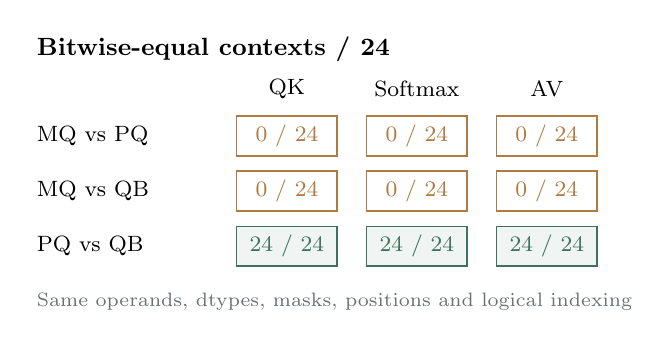
\begin{tikzpicture}[x=1cm,y=1cm,font=\footnotesize]
\node[anchor=west,font=\bfseries\small] at (0,2.65) {Bitwise-equal contexts / 24};
\foreach \x/\t in {3.30/QK,4.95/Softmax,6.60/AV}\node at (\x,2.15) {\t};
\foreach \y/\t in {1.55/MQ vs PQ,.85/MQ vs QB,.15/PQ vs QB}\node[anchor=west] at (0,\y) {\t};
\foreach \y in {1.55,.85}{\foreach \x in {3.30,4.95,6.60}{
 \draw[draft,line width=.65pt] (\x-.64,\y-.25) rectangle (\x+.64,\y+.25);
 \node[text=draft] at (\x,\y) {0 / 24};}}
\foreach \x in {3.30,4.95,6.60}{\draw[qualified,line width=.65pt,fill=qualified!8] (\x-.64,-.10) rectangle (\x+.64,.40);\node[text=qualified] at (\x,.15) {24 / 24};}
\node[anchor=west,text=aux,font=\scriptsize] at (0,-.55) {Same operands, dtypes, masks, positions and logical indexing};
\end{tikzpicture}

\caption{Fixed-input CUDA attention replay. Entries count contexts with bitwise-equal outputs out of 24. These are sampled layer-0 prefill/continuation contexts, not 24 independent model shapes. PQ/QB correspondence does not establish a general device reduction-order theorem.}
\label{fig:numeric}
\end{figure}

The result is stronger than agreement of final token IDs and narrower than global determinism. The experiment does not prove which CUDA kernel, reduction tree or library algorithm generated the correspondence: runtime operations and tensor geometry were recorded, but full kernel scheduling was unavailable. It also does not establish that this one layer mediates every complete-output recovery. In particular, some prefill captures share early prefixes; their numerical agreement is not additional independent generalization. We therefore state the mechanism as \emph{observed bitwise attention correspondence between QB and PQ on the sampled identical-input contexts}.

\subsection{Three-family complete-output qualification}
The larger confirmation~\cite{rtxconfirm} gives a separate test of decoder behavior. For each family, all 240 repeated outputs of $R$, $M_3$ and $C_3$ meet the complete registered endpoint. The unconstrained matched-capacity target-only path $M_0$ fails on 50/240 Qwen3, 140/240 SmolLM2 and 90/240 Llama requests (Table~\ref{tab:qual}). These failures are repeat observations over 5, 14 and 9 distinct tasks respectively, not independent failure trials. The contrast shows that merely using the target-only batched configuration is not sufficient for the chosen reference.

\begin{table}[t]\centering\small
\caption{Larger confirmation: matching complete endpoints /240 requests per arm. $M_0$ is unconstrained UB4. The $R_{\rm prod}$ values are independent of $M_0$ even when their counts coincide.}
\label{tab:qual}
\begin{tabular}{@{}lrrr@{}}\toprule
Arm & Qwen3 & SmolLM2 & Llama\\\midrule
$R$ &240&240&240\\
$M_0$ &190&100&150\\
$M_3$ &240&240&240\\
$C_3$ &240&240&240\\
$R_{\rm prod}$ &240&100&160\\\bottomrule
\end{tabular}
\end{table}

The engineering-selected ordinary $R_{\rm prod}$ keeps UB1 for Qwen3 and uses UB512 for the other two families. On the confirmation panel, SmolLM2 and Llama fail the registered reference in 140 and 80 requests respectively. Their ordinary-production comparisons cannot be promoted to qualified lossless speedups. Selection on exposed engineering tasks does not exempt a configuration from later qualification.

In the seven-arm repair campaign, every arm in every family completes and qualifies 96/96 outputs. Thus the direct PQ/QB/GS costs compare identical registered outputs within each family and task. This new result supplies cross-family implementation evidence while retaining the historical minimality boundary: it does not show that mask3 is minimal on all three families or that every unseen input will agree.

\subsection{The cost of the repair implementation}
Table~\ref{tab:cost} reports all 21 primary comparison estimates. QB is less expensive in aggregate than PQ for both target-only and speculative execution in each family. The speculative PQ/QB ratios are 1.044, 1.068 and 1.022 for Qwen3, SmolLM2 and Llama. The corresponding target-only ratios are 1.027, 1.038 and 1.013. These small differences are an implementation-level advantage under the tested conditions, not evidence of an order-of-magnitude improvement over a strong local alternative.

\begin{table*}[t]\centering\small
\caption{Complete same-reference request comparisons from the 12-task implementation campaign. Ratios above one favor the denominator; parentheses give the number of tasks on which the denominator is slower, out of 12. All 21 comparisons qualify. These are aggregate ratios, not latency-reduction percentages or kernel timings.}
\label{tab:cost}
\begin{tabular}{@{}lrrrrrrr@{}}\toprule
 & \multicolumn{2}{c}{Local repair} & \multicolumn{2}{c}{Global serialization} & Draft benefit & \multicolumn{2}{c}{Ordinary reference}\\
\cmidrule(lr){2-3}\cmidrule(lr){4-5}\cmidrule(lr){6-6}\cmidrule(l){7-8}
 & $M_{\PQ}/M_{\QB}$ & $C_{\PQ}/C_{\QB}$ & $M_{\GS}/M_{\QB}$ & $C_{\GS}/C_{\QB}$ & $M_{\QB}/C_{\QB}$ & $R/M_{\QB}$ & $R/C_{\QB}$\\\midrule
Qwen3 &1.027 (2)&1.044 (0)&1.330 (0)&2.144 (0)&1.144 (1)&1.334 (0)&1.526 (0)\\
SmolLM2 &1.038 (0)&1.068 (0)&1.366 (0)&1.463 (0)&0.634 (12)&1.370 (0)&0.868 (10)\\
Llama &1.013 (1)&1.022 (2)&1.412 (0)&2.176 (0)&1.117 (1)&1.426 (0)&1.592 (0)\\\bottomrule
\end{tabular}
\end{table*}

There are task-level exceptions. Qwen3's target-only PQ/QB comparison regresses on two GSM8K tasks; Llama regresses on one target-only task and two speculative tasks. No PQ/QB regression occurs in the SmolLM2 panel. The target-only comparisons also reverse direction between sessions: Qwen3's $M_{\PQ}/M_{\QB}$ is 0.971 and 1.085, and Llama's is 0.994 and 1.033. By contrast, $C_{\PQ}/C_{\QB}$ favors QB in both sessions for all three families (Supplement~S4). Thus the aggregate target-only advantage is session-sensitive; it should be distinguished from the consistently directed speculative session aggregates. Neither two adjacent sessions nor this small selected panel establishes long-term stability of a one-percent difference.

The distinction from global serialization is larger. GS/QB speculative ratios are 2.144, 1.463 and 2.176, and target-only ratios are 1.330, 1.366 and 1.412; every task favors QB in these comparisons. GS removes target-wide batching while QB constrains the attention organization only. The comparison supports the value of retaining other batched work under the common reference requirement. It does not isolate a measured fraction attributable to projection, FFN or graph launch overhead, since the experiments lack a completed component-time partition. Nor does it claim that GS is the fastest implementation of any external determinism method.

\begin{figure*}[t]
\centering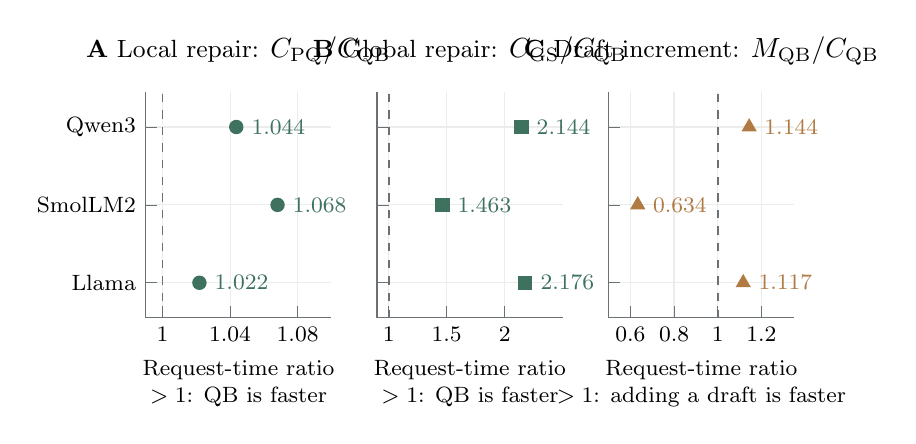
\begin{tikzpicture}
\pgfplotsset{repairaxis/.style={
 width=.325\textwidth,height=4.45cm,
 title style={font=\small},
 ymin=.55,ymax=3.45,ytick={1,2,3},
 tick label style={font=\footnotesize},
 xlabel style={font=\footnotesize,align=center},
 axis lines*=left,axis line style={aux,line width=.45pt},
 tick style={aux},grid=major,grid style={gray!15},
 point meta=explicit symbolic,
 every node near coord/.append style={font=\footnotesize,xshift=2pt},
}}
\begin{axis}[repairaxis,name=pq,
 title={\textbf{A} Local repair: {\normalsize $C_{\PQ}/C_{\QB}$}},
 xmin=.99,xmax=1.10,yticklabels={Llama,SmolLM2,Qwen3},
 xtick={1,1.04,1.08},xlabel={Request-time ratio\\$>1$: QB is faster}]
\addplot[aux,dashed,line width=.6pt] coordinates {(1,.55)(1,3.45)};
\addplot[only marks,mark=*,mark size=2.4pt,qualified,
 nodes near coords,nodes near coords align={right}]
 coordinates {(1.043676,3) [1.044] (1.068111,2) [1.068] (1.021848,1) [1.022]};
\end{axis}
\begin{axis}[repairaxis,at={(pq.east)},anchor=west,xshift=.58cm,name=gs,
 title={\textbf{B} Global repair: {\normalsize $C_{\GS}/C_{\QB}$}},
 xmin=.90,xmax=2.50,yticklabels={,,},
 xtick={1,1.5,2},xlabel={Request-time ratio\\$>1$: QB is faster}]
\addplot[aux,dashed,line width=.6pt] coordinates {(1,.55)(1,3.45)};
\addplot[only marks,mark=square*,mark size=2.4pt,qualified,
 nodes near coords,nodes near coords align={right}]
 coordinates {(2.143525,3) [2.144] (1.462530,2) [1.463] (2.175941,1) [2.176]};
\end{axis}
\begin{axis}[repairaxis,at={(gs.east)},anchor=west,xshift=.58cm,
 title={\textbf{C} Draft increment: {\normalsize $M_{\QB}/C_{\QB}$}},
 xmin=.50,xmax=1.35,yticklabels={,,},
 xtick={.6,.8,1,1.2},xlabel={Request-time ratio\\$>1$: adding a draft is faster}]
\addplot[aux,dashed,line width=.6pt] coordinates {(1,.55)(1,3.45)};
\addplot[only marks,mark=triangle*,mark size=2.8pt,draft,
 nodes near coords,nodes near coords align={right}]
 coordinates {(1.143749,3) [1.144] (.633948,2) [0.634] (1.116620,1) [1.117]};
\end{axis}
\end{tikzpicture}

\caption{Repair efficiency and speculation are different comparisons. Panels A/B: PQ/QB and GS/QB ratios with a draft; both compare qualified repairs. Panel C: adding a draft to the QB target-only path. Axis ranges differ across panels. Points are reported aggregate request ratios; no unmeasured confidence intervals are drawn. SmolLM2 benefits from QB over both repair alternatives while still losing to its own draft-free QB path.}
\label{fig:costfig}
\end{figure*}

\subsection{Adding a draft after repair}
$M_{\QB}/C_{\QB}$ measures the net effect of adding the complete speculative protocol to an already repaired target path. It is 1.144 for Qwen3 and 1.117 for Llama, with one slower task in each, but 0.634 for SmolLM2, with all 12 tasks slower. The last value corresponds to about 1.58 times the target-only request duration; it is not a small failure to capture an otherwise large gain. Nevertheless, $C_{\QB}$ is still cheaper than $C_{\PQ}$ and $C_{\GS}$ for SmolLM2. This is direct evidence that repair efficiency and speculative profitability must be stated independently.

The ordinary comparisons answer another question. In this same campaign, $R/M_{\QB}$ is 1.334, 1.370 and 1.426, while $R/C_{\QB}$ is 1.526, 0.868 and 1.592. Changes to target prefill/capacity and layout contribute jointly to ordinary-versus-matched comparisons. Those ratios cannot be attributed entirely to attention repair, and the multiplication with $M/C$ is an estimator identity rather than causal component accounting. The paper's method claim rests primarily on PQ/QB and GS/QB, not on labeling the full ordinary-to-candidate gain as speculative acceleration.

The larger 24-task confirmation has the same qualitative split: $M_3/C_3$ equals 1.135 for Qwen3, 0.607 for SmolLM2 and 1.072 for Llama, with 0/24, 24/24 and 4/24 regressions. Its ordinary-to-matched ratios are 1.383, 1.444 and 1.501. These are supporting results from a different campaign, not successive software-version speedups. Likewise the historical Qwen3 ratio 1.742 versus ordinary and 1.035 versus matched target-only remains in the supplement with its original panel, timer and round reversal; it is not substituted for the new campaign's numbers.

\subsection{Why work proxies are not enough}
A draft can reduce high-level target callers without reducing physical work proportionally. In a historical fixed-UB4 experiment~\cite{history}, widening $k$ from 3 to 7 preserved the endpoint but reduced relative speed to 0.829 in the generation interval and 0.890 in the request interval. Separate captured work sessions showed fewer target continuation callers but more micrographs, and a larger increase in proposed than accepted draft tokens. Those instrumentation counters cannot be divided by separately measured wall time to create a kernel profile.

Acceptance and query width describe workload generation. Their cost depends on the implementation's physical verification geometry and its measured request cost. We do not fit a break-even model to already observed performance or infer exclusive GPU stage times from asynchronous enqueue spans. The absence of such a model does not invalidate the observed same-reference implementation comparison; it limits predictive deployment claims.

\section{Execution-state and backend boundaries}
\label{sec:boundaries}
\subsection{A prefill intervention independent of the CUDA repair}
The B570 experiments use a distinct Vulkan frontend and a Llama-3.1-8B Q6\_K target. They address an applicability question raised by QB: can local attention control suffice when upstream projections and retained state depend on prefill organization? The experiments intervene on prefill partitions and boundary state while keeping single-query continuation. They diagnose that boundary independently of the CUDA repair; QB itself is not evaluated on Vulkan.

The original intervention~\cite{bpartition} holds a UB512/capacity 1 target context fixed. Arm A submits the full prompt in one prefill caller; B submits 128 tokens and the remainder. Arm C uses UB128 with one caller that the native runtime internally partitions. All arms request logits only for the final absolute prompt position; B's intermediate call requests none. Positions remain contiguous, and subsequent sampling and pending-token consumption are natural. For a 161-token prompt, actual physical widths are 161 in A and 128+33 in B/C. For 133 tokens the remainder is 5.

On the two exposed affected tasks, B reproduces C's full output and its initial full FP32 logits and source-defined sequence KV byte-for-byte, while A differs at generated indices 47 and 81. Two longer stable controls have different A/B numerical states but identical output. Synthetic prefixes of length 127 and 128 are unchanged, while a 129-token prefix differs at output 57. Thus exceeding 128 does not imply output divergence, and observing different state does not imply a changed greedy decision. The causal statement is that the specific external partition intervention is sufficient to reproduce these output boundaries, including its inherent per-call scheduling behavior.

\subsection{Partition equivalence is not a universal threshold}
In the final follow-up~\cite{bfinal}, a fourth arm D uses UB128 and an explicit 128+remainder caller split. It agrees with B/C in the full initial FP32 vector, all 64 K/V tensors and complete endpoints across the seven inputs. A frozen 19-schedule sweep, measured with observation off and on, further separates partition classes (Figure~\ref{fig:partition}). For the 133-token task, 64+64+5 and 96+37 match A, 128+5 matches B/C, and 132+1 yields a third full endpoint whose first difference occurs at 40. Smaller chunks are therefore not monotonically closer to the UB128 reference. More generally, A/B differ despite sharing UB512, while B/C/D agree despite different UB settings. A capacity number alone does not specify the observed reference behavior: actual partitioning and the resulting numerical state must also be recorded.

\begin{figure}[t]
\centering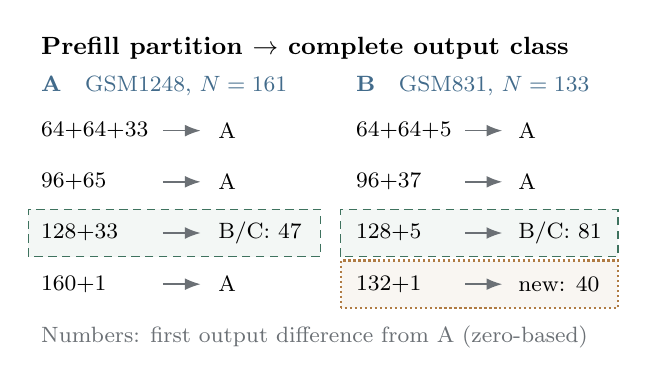
\begin{tikzpicture}[x=1cm,y=1cm,font=\footnotesize]
\node[anchor=west,font=\bfseries\small] at (0,3.35) {Prefill partition $\to$ complete output class};
\node[anchor=west,text=target] at (0,2.86) {\textbf{A}\quad GSM1248, $N=161$};
\node[anchor=west,text=target] at (4.0,2.86) {\textbf{B}\quad GSM831, $N=133$};
\begin{scope}[on background layer]
\fill[qualified!6] (-.04,.70) rectangle (3.67,1.30);
\fill[qualified!6] (3.93,.70) rectangle (7.45,1.30);
\fill[draft!7] (3.93,.05) rectangle (7.45,.65);
\end{scope}
\foreach \y/\lab/\out in {2.3/{64+64+33}/A,1.65/{96+65}/A,1.0/{128+33}/{B/C: 47},.35/{160+1}/A}{
 \node[anchor=west] at (0,\y) {\lab};\draw[flow] (1.67,\y)--(2.15,\y);\node[anchor=west] at (2.25,\y) {\out};}
\foreach \y/\lab/\out in {2.3/{64+64+5}/A,1.65/{96+37}/A,1.0/{128+5}/{B/C: 81},.35/{132+1}/{new: 40}}{
 \node[anchor=west] at (4.0,\y) {\lab};\draw[flow] (5.51,\y)--(5.98,\y);\node[anchor=west] at (6.06,\y) {\out};}
\draw[qualified,densely dashed] (-.04,.70) rectangle (3.67,1.30);
\draw[qualified,densely dashed] (3.93,.70) rectangle (7.45,1.30);
\draw[draft,densely dotted,line width=.8pt] (3.93,.05) rectangle (7.45,.65);
\node[anchor=west,text=aux,font=\footnotesize] at (0,-.32) {Numbers: first output difference from A (zero-based)};
\end{tikzpicture}

\caption{Observed partition/output classes for two exposed Vulkan inputs. A denotes whole UB512 prefill and B/C the 128-split reference class. Numbers indicate the first output difference from A; ``new'' is a third endpoint. Dashed outlines mark B/C and the dotted outline marks the third endpoint. This map does not imply a universal 128-token threshold. The follow-up sweep has the driver-hash preregistration limitation stated in the text.}
\label{fig:partition}
\end{figure}

The fourth-arm and sweep stages did not initially authenticate full external driver-body hashes, so they remain supplementary diagnostic evidence. Their later authentication does not retroactively repair that protocol gap. The independent source/payload audits still support the observed endpoints and tensor comparisons. We distinguish that narrower evidential value from a perfectly compliant new confirmation cohort.

\subsection{The numerical frontier can precede attention}
Source-aligned native observation finds equal A/B embeddings and admitted projection input activations, with B/C agreement at the named tensors. Differences are already present at the first-layer K/V projections for the 161-token task, and at Q/K/V for the 133-token task. The reported maximum absolute K/V differences for the first task are 0.052734375 and 0.0023193359375. For the second, Q differs only at logical positions 128--132, and K/V differ as well. This localizes a divergent projection frontier before later attention; the order in which sibling projections were listed is not evidence of a unique first-cause kernel.

Forty standalone operator calls compare full versus 128-split geometry on identical captured operands. Thirty-two pass native same-arm shams. RMS and the first task's Q-projection controls are bitwise invariant, while the admitted differing projection replays reproduce geometry sensitivity. All eight scale/MUL calls fail correspondence because their operands were captured after an in-place consumer had modified an aliased buffer. They are excluded, not counted as successful mechanism observations. Exact Vulkan shader, pipeline and dispatch identities remain unknown.

QB retains projection batching, so its portability depends on numerical differences outside the constrained attention graph. The CUDA qualification establishes suitability for that stack and panel. On B570, projection differences precede attention, and later continuations remain sensitive to retained-state differences. This earlier frontier can require constraints on state formation beyond the attention layout.

\subsection{A controlled retained-KV intervention}
Stage-Replay has already shown that transplanted KV can select a later suffix despite identical initial tokens~\cite{stagereplay}. Here, the final study tests states formed by fixed-precision partition interventions, using a boundary0 reconstruction admitted through own-path controls (Figure~\ref{fig:state}). Two prefill recipes provide $(KV_A,L_A)$ and $(KV_B,L_B)$, where $L$ is the complete initial FP32 logit vector. A clean common UB512 receiver restores sequence K/V content and positions, applies the identical native greedy sampler to the selected logits, reconstructs the empty generated prefix and pending-token obligations, and proceeds with single-query continuation. Sixteen own-path shams reproduce entire natural endpoints and retained-state checks before the cross is admitted.

\begin{figure}[t]
\centering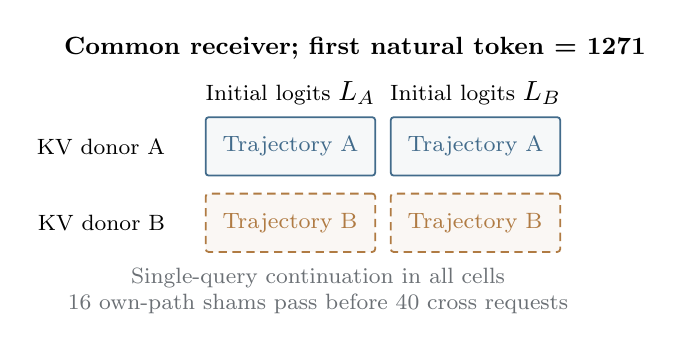
\begin{tikzpicture}[x=1cm,y=1cm,font=\footnotesize,
  box/.append style={font=\footnotesize,line width=.65pt,text width=1.8cm,minimum height=.74cm}]
\node[anchor=west,font=\bfseries\small] at (0,3.35) {Common receiver; first natural token = 1271};
\node at (3.0,2.78) {Initial logits {\normalsize $L_A$}};\node at (5.35,2.78) {Initial logits {\normalsize $L_B$}};
\node[anchor=east] at (1.53,2.1) {KV donor A};\node[anchor=east] at (1.53,1.13) {KV donor B};
\foreach \x in {3.0,5.35}{
 \node[box,draw=target,fill=target!5,text=target] at (\x,2.1) {Trajectory A};
 \node[box,draw=draft,fill=draft!6,text=draft,densely dashed] at (\x,1.13) {Trajectory B};}
\node[align=center,text=aux,font=\footnotesize] at (3.35,.26) {Single-query continuation in all cells\\16 own-path shams pass before 40 cross requests};
\end{tikzpicture}

\caption{Qualified boundary0 state cross on the two affected Vulkan tasks. Each cell gives the complete trajectory class. All initial logit vectors choose token 1271, making a logit-source swap a first-decision negative control. Changing the KV source changes the later suffix at indices 47/81. The two stable long controls remain output-invariant despite differing KV bytes.}
\label{fig:state}
\end{figure}

Forty cross requests cover the two affected inputs with three repetitions per cell and two stable long inputs with two. For the affected tasks,
\begin{equation}
Y(KV_A,L_A)=Y(KV_A,L_B)=Y_A,
\end{equation}
\begin{equation}
Y(KV_B,L_A)=Y(KV_B,L_B)=Y_B,
\end{equation}
with $Y_A\ne Y_B$ at the historical first-difference positions. All initial vectors choose token 1271, so the null logit-swap result does not establish that future logits are irrelevant. The positive intervention is conditional suffix sensitivity to the KV source under the common validated receiver contract. It neither proves universal causal necessity of KV nor implements arbitrary opaque state cloning. The stable controls retain the same full endpoint under both KV sources.

The projection replay and KV cross strengthen different links in the explanation. They do not isolate which individual layer, token or K-versus-V change accounts for the full effect. A claim that every projection perturbation is mediated exclusively through a particular KV subset would require additional interventions. The practical boundary is that constraining later calls to one-query geometry does not remove differences already carried by retained state. Choosing a local repair therefore requires checking both the numerical frontier and the state that crosses the constrained boundary.

\subsection{Physical verification and the cost boundary}
In the separate B570 speculative implementation, a logical $k=1$ verification caller with two rows executes two occupied width-one target micrographs, plus draft proposal and catch-up work. The physical-work study records this decomposition in 563 cycles across 11 completed candidate witnesses~\cite{bwork}. High measured acceptance therefore does not establish multiquery physical graph amortization. Micrographs are not shader launches, and their counts cannot assign a fraction of request time to a component.

The earlier 1,200-request B570 campaign~\cite{bcost} failed its frozen stock-reference qualification on two tasks. A separate post-hoc audit established that $R_{\rm prod}$, $M_{\rm match}$ and $C_{k 1}$ have identical full outputs on all 240 paired repetitions across 24 tasks~\cite{bpostaudit}. Their observed ratios, $R_{\rm prod}/C=0.719264$ and $M/C=0.727927$, describe negative same-output production-path economics; they do not repair the original stock gate. Every task regresses. No new latency benchmark or phase-time model is supplied by the later diagnostic experiments. Hardware timestamps are supported, but the pinned backend interface does not expose a qualified completed GPU timeline; continuous physical residency also remains unproved.

\section{Related work and limits}
\label{sec:limits}
\subsection{Relation to numerical-consistency methods}
Batch-invariant inference controls reductions in normalization, matrix multiplication and attention, including the split boundaries used for chunked prefill~\cite{thinkingmachines}. LayerCast studies sensitivity to batch size and hardware configuration, storing weights in 16-bit precision while computing in FP32~\cite{layercast}. TBIK aligns intra- and inter-GPU reduction orders across tensor-parallel sizes~\cite{tbik}. Our method instead changes query/mask views and runtime phase/cache controls in a fixed quantized stack. It targets the registered ordinary reference without changing precision or rewriting backend arithmetic kernels; it does not establish invariance across tensor-parallel configurations.

LLM-42 combines fast execution with fixed-shape verification, rollback and consistent state maintenance~\cite{llm42}. Fixed shapes, selective constraints and reuse of existing kernels are therefore prior ideas. Our candidate directly changes the target attention graph without an extra numerical-consistency recovery replay. This architectural distinction does not establish a speed advantage over LLM-42. A historical adaptation encountered reference-contract mismatches and incomplete confirmation, so it supplies neither a qualified ranking nor evidence that the original system fails.

MarginGate uses margin-triggered selective verification~\cite{margingate}; our runtime applies a fixed, empirically qualified phase/layout recipe. Vosti specifies deterministic inference across batching, chunking, prefill/decode, query lengths and physical cache layouts using fixed kernel configurations and engine/cache invariants~\cite{vosti}. Vosti proves determinism under its stated assumptions; our evidence is finite qualification against a registered ordinary reference.

\subsection{Relation to cache and state diagnostics}
Stage-Replay uses fixed-prefix controls, bidirectional KV transplantation and a common suffix decoder; its transplants retain recipient boundary logits and require the same first suffix token~\cite{stagereplay}. Cache-carried divergence despite an identical initial token is thus prior work. Patodiya reports cache-state-dependent divergence in quantized serving, including cached and recomputed paths that are individually repeatable but disagree~\cite{cachestate}. A prior llama.cpp diagnostic also reports fixed-input Vulkan projection differences and a local correction that leaves whole-model divergence unresolved~\cite{vulkandiagnostic}; this is an engineering report, not a peer-reviewed guarantee.

Our B570 contribution is the partition intervention at fixed precision, the measured projection frontier and state reconstruction admitted through own-path shams. The main method contribution rests on the QB graph design and its in-stack same-reference cost comparisons. Neither shared concepts nor our finite checks establish portability. A common-contract comparison with a mature external implementation remains open.

\subsection{Relation to speculation economics}
The original speculative decoding result preserves a target sampling distribution under its algorithmic assumptions~\cite{leviathan2023}; reproducing a chosen finite-precision greedy path is an additional implementation requirement. Performance studies show why target verification cost and actual backend behavior matter beyond accepted-token counts~\cite{illusion,lossless}. We treat those insights as prior foundations. The new question here is the cost of alternative \emph{qualified repair implementations}, followed by the incremental cost of adding the speculative protocol on the repaired path.

The unrelated ACL work named HeteroSpec allocates verification using contextual heterogeneity~\cite{aclheterospec}. Our repository retains its historical project name, but this article uses a descriptive method title to avoid a naming collision. The scientific objectives and implementation contribution are distinct.

\subsection{Scope and threats to validity}
The structural mapping is reusable only when its stated tensor, stream, mask and head conditions hold. The numerical evidence is restricted to pinned non-flash CUDA graphs, small occupied query widths and the tested model conversions. Three families do not establish all architectures; shared backend components reduce their independence. Projection batching retained by QB may be inappropriate on another stack, as the Vulkan frontier illustrates. Neither operator replay nor mask enumeration supplies an all-input numerical-preservation theorem.

The complete-output studies use finite cap128 windows and greedy sampling. They do not establish stochastic distribution preservation for the implementation, long-context stability, concurrent throughput, energy efficiency, production tail latency or arbitrary state-restoration boundaries. Selected sensitive diagnostic inputs are appropriate for mechanism tests but cannot estimate the prevalence of divergence. Synthetic prefix experiments preserve exact native IDs, not natural task semantics.

Request medians and balanced order reduce some measurement variation but do not remove thermal, clock, operating-system or session confounding. Adjacent sessions cannot justify cross-date confidence intervals. The small PQ/QB advantages, target-only session reversals and task regressions should temper deployment claims; larger GS/QB differences do not remove the need for a fair local comparator. No fitted cost model or observer-overhead subtraction is used. Lack of continuous residency proof limits hardware-residency assertions rather than retroactively erasing the measured output and request observations.

Provenance failures are not silently repaired. The driver-freeze gap, rejected scale replays, resource amendments, missing historical slots and differing endpoint contracts remain explicit. The supplement preserves the historical evidence destinations and distinguishes reported-value checks in this reconstruction from original-host raw-data audits. Before public release, external readers need an accessible source/evidence package and a documented path to the exact model assets; a private repository pointer alone is not a public reproducibility guarantee.

\section{Conclusion}
\label{sec:conclusion}
Attention query geometry can be controlled independently of target-wide batching. Our phase-scoped layout combines query/mask views, native K/V and GQA semantics, ordered recombination, and phase-aware graph reuse. Fixed-input CUDA replay establishes sampled bitwise PQ/QB correspondence; separate three-family experiments establish complete registered-output qualification. QB lowers aggregate request cost relative to PQ and global serialization under that common reference. Target-only PQ/QB costs remain session-sensitive for Qwen3 and Llama, and adding a draft is unprofitable for SmolLM2.

Vulkan interventions delimit the design's scope. Actual prefill partitions can change projections and retained state, and a qualified KV-source intervention changes later output despite one-query continuation. These findings support validation of state formation and the complete execution path. They establish neither a universal attention-only repair nor an unrestricted determinism guarantee. The method's contribution is its specified graph design, measured same-reference repair costs and tested applicability boundaries.

\section*{Data and code availability}
The implementation and experiment-specific records are identified by the commit-pinned companion sources. The accompanying author package supplies manuscript sources, reported-value data, a claim-to-evidence map and reconstruction checks. Full native captures and execution records remain in the study repository; some source capsules, binaries and model assets require separate access. The package distinguishes its reported-value checks from the original hosts' raw-data audits.
\section*{Declaration of generative AI and AI-assisted technologies}
AI-assisted tools supported code development, analysis and manuscript preparation. In this revision, OpenAI Codex (GPT-6, OpenAI; October 2026) assisted with reported-value checks, editable TikZ/PGFPlots figure code, source packaging and language editing, including a humanizer style pass. The reported measurements were not generated or replaced by AI. The author is responsible for verifying the analyses, references, figures and final text before submission.
\bibliographystyle{psql-num}
\bibliography{references}
\end{document}
